% \documentclass{cumcmthesis}
\documentclass[withoutpreface,bwprint]{cumcmthesis} %去掉封面与编号页,电子版提交的时候使用。


\usepackage[framemethod=TikZ]{mdframed}
\usepackage{tikz}
\usepackage{tikz-3dplot}
\usepackage{gbt7714}
\usepackage{url}   % 网页链接
\usepackage{subcaption} % 子标题

\usetikzlibrary{positioning, shapes.geometric}

\title{基于SPO-GA混合算法的定日镜场布局优化设计}
\tihao{A}
\baominghao{202317225001}
\schoolname{湖北文理学院}
\membera{廖嘉旺}
\memberb{董克旋}
\memberc{彭山}
\supervisor{孙成娇}
\yearinput{2023}
\monthinput{09}
\dayinput{10}

\begin{document}

\maketitle

\begin{abstract}
    利用塔式太阳能光热发电站发电是一种低碳环保的新型清洁能源技术。本文针对塔式电站定日镜场布局的优化设计的问题,基于定日镜聚光模型,阴影挡光效率理论模型 ,镜场布局模型,粒子群优化算法以及遗传算法建立了数学模型,为研究定日镜的物理模型以及优化结构设计提供了理论支持,有效提升定日镜场的光热效率响应国家节能减排,低碳环保的目标。

    对于问题一:主要解决了两个问题,一是建立太阳位置模型,计算出各个时间的太阳高度角和方位角,再根据定日镜聚光模型中的旋转矩阵计算出定日镜法方位角和高度角。二是利用光线追踪法以及光的反射定律模拟出了光线的反射路径,求得了定日镜的法线向量。之后计算出四个效率参数。其中,在计算遮挡效率时,运用python语言,对光线进行模拟跟踪得到定日镜的可视化图像。最后的效率参数都通过计算并填入了表格。

    对于问题二:建立定日镜场的布局结构优化模型,并对参数进行了的初始化,首先建立基本的布局结构模型作为本文优化的基础,确定约束和镜场大小的界限,其次在通过粒子群优化算法得到优化后的镜场结构布局,并得出了粒子群在迭代过程中稳定后的收敛位置,之后用python进行数据可视化处理。得到了定日镜场优化布局后的图像。最后将定日镜场参数按模板规定的格式保存到了result2.xlsx 文件中。

    结对于问题三:建立粒子群优化和遗传混合算法(PSO-GA)。在问题二的模型上进一步优化处理。并得到了优化后的定日镜场分布图像,将定日镜场的参数按规定的格式保存到了result3.xlsx 文件中。

    最后对本文建立的模型进行推广和评价,综合评价模型。

    \keywords{定日镜场布局优化\quad 粒子群算法\quad 遗传算法\quad 混合算法}
\end{abstract}

\section{问题重述}

\subsection{问题背景}

塔式太阳能定日镜场是一种低碳环保的新型清洁能源技术\cite{许利华2020},也是我国为实现“碳达峰”和“碳中和”目标而采取的重要举措。定日镜是塔式太阳能光热发电站收集阳光的基本组件,由可纵向旋转的横轴和水平旋转的水平轴构成。通过控制两轴的旋转角度,可以有效利用定日镜将太阳光反射聚焦到吸收塔顶端的集热器中心。集热器再通过汇聚的阳光去加热其中的导热介质,并以热能的形式储存起来,最终转换成可使用的电能。因此,优化设计镜场结构,提高光电转换效率对定日镜场至关重要。

\subsection{问题提出}

吸收塔的高度为80m,顶部建有集热器。集热器是一个直径为7m、高度为8m的圆柱形受光式集热器。同时,在吸收塔周围100m的范围内,需要留出空地用于建造厂房,安装发电、储能和控制设备。定日镜的形状为平面矩形,通常镜面宽度大于镜面高度,边长在2m至8m之间,安装高度在2m至6m之间。同时,需要确保定日镜在追踪太阳旋转时不会接触地面。相邻定日镜底座中心之间的距离至少要比镜面宽度多5m以上。现计划在中心位于东经98.5°,北纬39.4°,海拔3000m的圆形区域建设一个圆形定日镜场。为了解决以下问题,我们以圆形定日镜场区域中心为坐标原点建立笛卡尔坐标系,建立数学模型。


\begin{itemize}
    \item { \textbf{问题一:}根据给定的定日镜尺寸为6m $\times$ 6m,安装高度为4m,将吸收塔建于该圆形区域的太阳直射中心,结合附件中给定的定日镜中心位置,计算定日镜场的平均光学效率、年平均输出热效率以及单位镜面面积年平均输出热功率。 }
    \item { \textbf{问题二:}要求定日镜场的额定年平均输出热功率达到60MW,并保持所有定日镜尺寸与安装高度相同。在此条件下设计定日镜场的以下参数:吸收塔的位置坐标、定日镜尺寸、安装高度、定日镜数目以及定日镜位置,以使得单位镜面面积年平均输出热功率最大化。 }
    \item { \textbf{问题三:}要求定日镜尺寸与安装高度可以不同。在定日镜场的平均输出热效率达到60MW的条件下,重新设计定日镜场的各个参数,包括定日镜尺寸、安装高度等,以使得单位镜面面积年平均输出热功率尽量大。 }
\end{itemize}

\section{问题分析}

本文的研究对象是定日镜场,研究内容为定日镜的安装参数和布局结构对光热效率的影响关系,该问题描述了定日镜在不同安装高度,定日镜尺寸以及吸收塔与定日镜不同布局的变化特点下提出的不同要求,达到优化的目的。

\subsection{对问题一的分析}

问题一是基于在固定参数的定日镜场条件下,要求计算关于定日镜场的各个效率,由附录给出的计算效率的公式可以求出在固定地点在不同时间点的太阳高度角和方位角,由此我们建立太阳模型和定日镜聚光模型可以进一步求出定日镜的高度角和方位角,从而得出光线的入射,反射及关系。再利用光线跟踪法模拟出光线的反射路径,镜面遮挡的效率,从而解出所有效率参数,进而可解出定日镜光学效率和输出热功率。图\ref{fig:quesion1_flow}为问题一的分析流程图。

\begin{figure}[hptb]
    \centering
    \begin{tikzpicture}
        \node[] (center){};
        \node[draw,above= of center] (box 0) {计算太阳的高度角与方位角};
        \node[draw,left=of center] (box 1) {太阳位置模型};
        \node[draw,right=of center] (box 2) {定日镜聚光模型};
        \node[draw,below =of center] (box 3) {求出定日镜相关坐标与参数};
        \node[draw,below =of box 3] (box 4) {光线追踪法};

        \node[below=of box 4] (temp){};

        \node[draw,right=of temp] (box 5) {遮挡效率};
        \node[draw,right=of box 5] (box 6) {余弦效率};
        \node[draw,left=of temp] (box 7) {大气透射效率};
        \node[draw,left=of box 7] (box 8) {截断效率};

        \node[draw,below = of temp] (box 9) {定日镜光学效率};

        \draw[->] (box 0) -- (box 1);
        \draw[->] (box 0) -- (box 2);

        \draw[->] (box 1) -- (box 3);
        \draw[->] (box 2) -- (box 3);
        \draw[->] (box 3) -- (box 4);


        \foreach \i in {5,6,...,8}
        \draw[->] (box 4) -- (box \i);
        \foreach \i in {5,6,...,8}
        \draw[->] (box \i) -- (box 9);

    \end{tikzpicture}
    \caption{问题一分析流程图}
    \label{fig:quesion1_flow}
\end{figure}

\subsection{对问题二的分析}

分析问题二,设计定日镜的各种参数和吸收塔的位置坐标,要求在定日镜场的额定年平均输出热功率达到60 MW的情况下,使得单位镜 面面积年平均输出热功率尽量大。这是一个最优化问题,粒子群模型是一种适合解决这种多参数优化问题的方法。首先我们要找到参数与参数之间的联系,然后我们要找到约束条件,确定目标函数和决策变量,再基于单目标多约束的粒子群优化算法得出结果。其中参数的确定需要定日镜场的初始化布局。

\subsection{对问题三的分析}

问题三与问题二在模型建立和求解上是相同的类型,其本质也是最优化问题,使得镜面面积年平均输出热功率大。区别是模型的决策变量增加。用问题二中的粒子群算法求解的时间复杂度高,因此我们引进新的启发式模型,与粒子群优化算法结合,在问题二的基础上进行优化。

\section{模型假设}

\begin{assumption}
    假设在本文研究检测的时间段内不会出现极端天气对定日镜聚光造成影响。
\end{assumption}

\begin{assumption}
    假设所有定日镜在运行正常,不需要维护。
\end{assumption}


\section{符号说明}

本文中提出的符号如表\ref{tab:notation}所示。

\begin{table}[hptb]
    \centering
    \caption{符号说明}
    \label{tab:notation}
    \begin{tabular}{@{}ccc@{}}
        \toprule
        序号 & 符号           & 说明           \\ \midrule
        1  & $\alpha_{s}$ & 太阳高度角        \\
        2  & $\gamma_{s}$ & 太阳方位角        \\
        3  & $h_{j}$      & 定日镜高度角       \\
        4  & $\theta_{j}$ & 定日镜方位角       \\
        5  & $\vec{s}$    & 太阳光入射的光线     \\
        6  & $\vec{r}$    & 太阳光经定日镜的反射光线 \\
        7  & $\eta_{k}$   & 第k面定日镜的光学效率  \\ \bottomrule
    \end{tabular}
\end{table}

\section{模型建立和求解说明}

\subsection{问题一:结合光线跟踪法,计算所求光学效率}

针对问题一,需要通过计算太阳高度角和方位角进而来计算该定日镜场的年平均光学率、年平均输出热功率,以及单位镜面面积年平均输出热功。分析题目可知计算平均光学效率需要计算平均余弦效率,平均阴影遮挡效率,平均截断效率以及大气透射率。

\subsubsection{太阳位置模型}

\textbf{太阳赤纬角的计算} \space 太阳赤纬角是指地球的公转轨道面与赤道面的夹角,可以通过蔡志杰提出的式\ref{eq:delta}计算。

\begin{equation}
    sin\delta=sin\frac{2\pi D}{365}sin(\frac{2\pi}{360}23.45) \label{eq:delta}
\end{equation}

其中$D$是以春分作为第0天起算的天数。

\textbf{太阳时角的计算} \space 太阳时角$\omega$可由式\ref{eq:omega}计算得出。

\begin{equation}
    \omega=\frac{\pi}{12}(ST-12) \label{eq:omega}
\end{equation}

其中$ST$ 为当地时间的24小时时制。

\textbf{太阳高度角和方位角的计算}

已知以上两项和当地纬度$\phi$,太阳高度角和方位角可以由式\ref{eq:alpha}、\ref{eq:gamma}计算。

\begin{equation}
    sin\alpha_{s} = cos\delta cos\varphi cos\omega + sin\delta sin\varphi \label{eq:alpha}
\end{equation}

\begin{equation}
    cos\gamma_{s}=\frac{sin\delta-sin\alpha_{s}sin\varphi}{cos\alpha_{s}cos\varphi} \label{eq:gamma}
\end{equation}

其中维度为北时为正,南纬是为负。

通过公式的计算和计算机的验证,我们得到了60个时间点的太阳高度角和方位角,作图后如图所示。

\begin{figure}
    \centering
    \resizebox{\textwidth}{!}{
        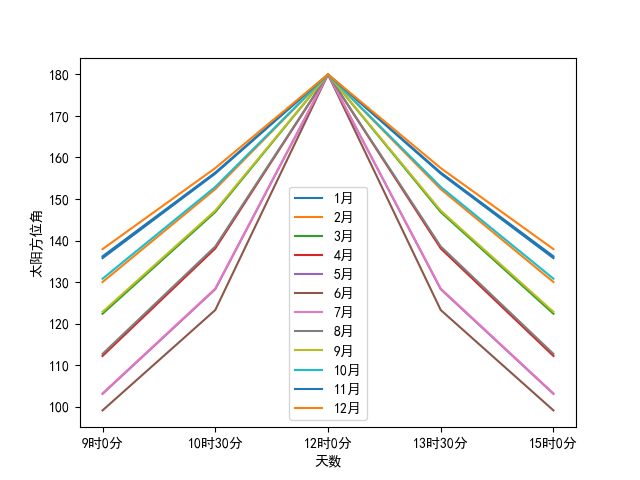
\includegraphics{../A题/太阳方位角.png}
    }
    \caption{太阳方位角}
\end{figure}

\begin{figure}
    \centering
    \resizebox{\textwidth}{!}{
        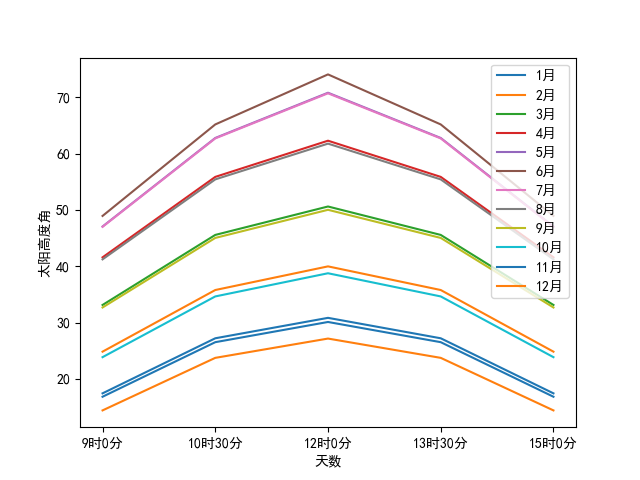
\includegraphics{../A题/太阳高度角.png}
    }
    \caption{太阳高度角}
\end{figure}

\textbf{非平行太阳光的锥角} \space 太阳光并非平行光线,而是具有一定锥角的一束锥形光线,因此太阳光总是以光锥的形式到达地球表面,并以光斑的形状呈现出来。根据反射原理,光线反射到集热器上的光线也呈光斑形状,在定日镜场中,有离集热器较近和较远的定日镜,光斑的面积也会因距离的不同而变化,由于以上原因造成了反射光线不能全部落在集热器的接收表面,从而造成了一定的光溢出。

\textbf{非平行太阳光的向量表示} \space 太阳光线的方向随着时间的变化而变化,为了之后的计算方便,我们先建立镜场坐标系并确定太阳光锥的主入射光线$\vec{s}=(S_{x},S_{y},S_{z})$,可由式\ref{eq:vector_of_sun_cone}计算得出,在太阳体积是地球的 130 倍的前提下,同一地方接收到的太阳光可视为平行光,因此我们可以用太阳的高度角$\alpha_{s}$和方位角$\gamma_{s}$来表达太阳光线,如图\ref{fig:vector_of_sun_cone}。

\begin{figure}[hptb]
    \centering
    \tdplotsetmaincoords{70}{30}
    \begin{tikzpicture}[tdplot_main_coords, scale=2]

        % draw the axes
        \draw[thick,->] (0,0,0) -- (2,0,0) node[anchor=north east]{$x$};
        \draw[thick,->] (0,0,0) -- (0,2,0) node[anchor=north west]{$y$};
        \draw[thick,->] (0,0,0) -- (0,0,2) node[anchor=south]{$z$};

        % point (1,1,1.5)
        \node (P) at (1,1,1.5) [circle,fill,inner sep=1pt,label={below right:$P$}]{};
        \draw[-latex] (0,0,0) -- (P);

        % project (1,1,1.5)
        \draw[dashed] (1,1,1.5) -- (1,1,0) -- (0,0,0);
        \draw[dashed] (1,0,0) -- (1,1,0) -- (0,1,0);

        % angle theta
        \tdplotdrawarc[-latex]{(0,0,0)}{0.3}{45}{90}{anchor=north}{$\theta_s$}

        % draw the rays
        \foreach \i in {0, 0.5 ,...,2}
        \draw[-latex] (\i,2.5,1) -- (\i,1.5,0.5);

        % draw a sun
        \node at (1.5,1.5,2) [circle,fill=orange,inner sep=5pt]{};
    \end{tikzpicture}
    \caption{太阳光锥的向量表示}
    \label{fig:vector_of_sun_cone}
\end{figure}

\begin{equation}
    \vec{s}=(S_{x},S_{y},S_{z})=(cos\alpha_{s}cos\gamma_{s},cos\alpha_{s}sin\gamma_{s},sin\alpha_{s}) \label{eq:vector_of_sun_cone}
\end{equation}

\subsubsection{定日镜聚光模型}
由于太阳光线不断的变化,需要转动定日镜对太阳光进行聚光。在定日镜聚光的过程中,要考虑定日镜的跟踪方法,在不同时刻还需根据太阳和目标点的相对位置调整定日镜姿态。根据题目所述,定日镜由纵向转轴和水平转轴组成,可以控制反射镜的方位角和俯仰角。因此我们选择高度角-方位角跟踪方式[塔式调养能定日镜聚光成像策略研究]使光线的反射率最大化。

\textbf{建立定日镜坐标系} \space 为了实现较为精确的跟踪方法,我们对每面定日镜都引入一新的坐标系,方便对各个顶点的描述,如下图所示,我们以定日镜的几何中心为坐标原点,将平行于横轴的两条边命名为LA,垂直与横轴的两条边命名为LB,过原点平行于LA的为y轴,偏北为正,过原点平行于LB的为x轴,偏东为正,过原点垂直于地面为z轴,向外指为正。

\ref{fig:coordinate_of_mirror}

% \tdplotsetrotatedcoords{0}{0}{0}
\begin{figure}[hptb]
    \centering
    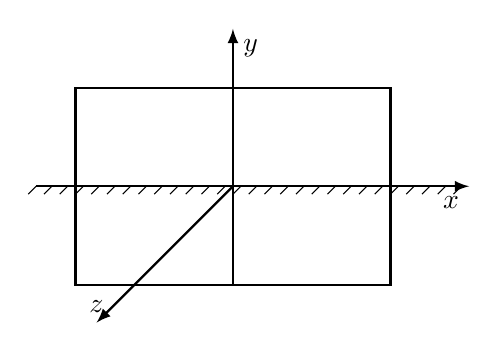
\begin{tikzpicture}
        % draw the axe
        % \draw[thick] (-2,0,0) -- (2,0,0);
        % \draw[thick] (0,0,0) -- (0,0.5,0);
        % \draw[dashed,thick] (0,0.5,0) -- (0,3,0);

        % \node at (0,3,0) [circle,fill,inner sep=1pt,label={below right:$O$}]{};

        % \begin{scope}
        \draw[thick,-latex] (-2.5,0,0) -- (3,0,0) node[anchor=north east]{$x$};
        \draw[thick,-latex] (0,-1.25,0) -- (0,2,0) node[anchor=north west]{$y$};
        \draw[thick,-latex] (0,0,0) -- (0,0,4.5) node[anchor=south]{$z$};

        \draw[thick] (2,1.25,0) -- (2,-1.25,0) --  (-2,-1.25,0) --(-2,1.25,0)-- cycle;
        % \end{scope}

        % draw the wall
        \foreach \i in {-2.5, -2.3 ,...,3}
        \draw[] (\i,0,0) -- (\i-0.1,-0.1,0) ;
    \end{tikzpicture}
    \caption{定日镜坐标系}
    \label{fig:coordinate_of_mirror}
\end{figure}

\textbf{坐标旋转矩阵} \space 若假设初始定日镜状态的镜面法向量为$\vec{z}$=(0,0,1),则在进行定日镜聚光的光线跟踪时,定日镜会通过旋转转轴来调整定日镜姿态,从而使定日镜镜面法向量发生改变,与太阳角度定义类似,现引入定日镜的高度角$h_{j}$和定日镜的方位角$\theta_{j}$,通过对坐标进行旋转矩阵的变换来达到跟踪的结果。下面是光线跟踪时出现的两种旋转情况:\ref{fig:rotate_x}

绕x轴旋转时,旋转矩阵为:

\begin{equation}
    R_{x}(\alpha)=\left[\begin{array}{ccc}
            1 & 0         & 0          \\
            0 & cos\alpha & -sin\alpha \\
            0 & sin\alpha & cos\alpha
        \end{array}\right] \label{eq:rotate_x}
\end{equation}

\begin{figure}[hptb]
    \centering

    \tdplotsetmaincoords{45}{115}
    \begin{tikzpicture}[tdplot_main_coords, scale=2]
        % draw the axes
        \draw[thick,->] (0,0,0) -- (2,0,0) node[anchor=north east]{$x$};
        \draw[thick,->] (0,0,0) -- (0,2,0) node[anchor=north west]{$y$};
        \draw[thick,->] (0,0,0) -- (0,0,2) node[anchor=south]{$z$};

        % draw point 
        \node at (1.5,0,2) [circle,fill,inner sep=1.5pt,label={above right:$Z'$}]{};
        \node at (0,1,2) [circle,fill,inner sep=1.5pt,label={right:$Y'$}]{};

        % draw the arrow
        \draw[dashed,-latex] (0,0,0) -- (1.5,0,2);
        \draw[dashed,-latex] (0,0,0) -- (0,1,2);

        \begin{scope}[canvas is yz plane at x=0]
            \tdplotdrawarc[-latex]{(0,0)}{1}{0}{60}{}{}
            \node at (0.8,0.6) [label={right:$\alpha$}]{};
        \end{scope}

        \begin{scope}[canvas is yz plane at x=0.8]
            \tdplotdrawarc[-latex]{(0,0)}{0.5}{0}{180}{}{}
            \node at (0,0) [label={left:$\alpha$}]{};
        \end{scope}

        \begin{scope}[canvas is xz plane at y=0]
            \tdplotdrawarc[-latex,label={right:$\alpha$}]{(0,0)}{1.2}{90}{52}{}{}
            \node at (1.5,2.5) [label={right:$\alpha$}]{};
        \end{scope}
    \end{tikzpicture}

    \caption{绕x轴旋转示意图}
    \label{fig:rotate_x}
\end{figure}


绕y轴旋转时,旋转矩阵为:

\begin{equation}
    R_{y}(\alpha)=\left[\begin{array}{ccc}
            cos\alpha  & 0 & sin\alpha \\
            0          & 1 & 0         \\
            -sin\alpha & 0 & cos\alpha
        \end{array}\right] \label{eq:rotate_y}
\end{equation}


绕z轴旋转时,旋转矩阵为:

\begin{equation}
    R_{z}(\alpha)=\left[\begin{array}{ccc}
            cos\alpha & -sin\alpha & 0 \\
            sin\alpha & cos\alpha  & 0 \\
            0         & 0          & 1
        \end{array}\right] \label{eq:rotate_z}
\end{equation}

在上述式子中$\alpha_{x},\alpha_{z}$均以逆时针旋转为正方向。通过旋转矩阵,可以求出反射到镜面光线的法线。

为了方便量化定日镜的旋转角度,我们定义定日镜的法线方向与z轴方向的夹角为定日镜的高度角$h_{j}$,定日镜的法线投影与的 y 轴正向所成的逆时针夹角为定日镜的方位角,由几何关系与题目可知,为了使得太阳中心点发出的光线经定日镜中心反射后指向 集热器中心。太阳方位角的变化和定日镜的方位角变化是几乎相同的,即太阳的方位角$\gamma_{s}$与定日镜的方位角$\theta_{j}$相等。

\textbf{定日镜的聚光模型求解} \space 在上文中我们知道了太阳主光线的向量坐标表示,我们定义定日镜为理想模型即反射后的光线能够平整的反射到集热器。我们定义集热器表面中心B为$(x_{b},y_{b},z_{b})$,定日镜镜面中心O为$(x_{o},y_{o},z_{o})$,则反射向量为

\begin{equation}
    \vec{r}=\frac{(x_{b}-x_{c},y_{b}-y_{c},z_{b}-z_{c})}{\| \mathbf{d_{OB}} \|}
\end{equation}

由式\ref{eq:normal_vector}得出太阳光入射单位向量为

\begin{equation}
    \vec{s}=(-cosh_{s}cos\theta_{s},-cosh_{s}sin\theta_{s},-sinh_{s})
\end{equation}

由反射定律可以得到入射向量,反射向量和镜面法向量的关系:

\begin{equation}
    \vec{n}=\frac{-\vec{s}+\vec{r}}{\| \mathbf{{-\vec{s}+\vec{r}}\|}}
\end{equation}

联立上述式子,可得:

\begin{equation}
    R_{z}(\theta)\cdot R_{y}(\varphi)\cdot \vec{z}=\frac{(-cosh_{s}cos\theta_{s},-cosh_{s}sin\theta_{s},-sinh_{s})+\vec{r}}{\| \mathbf{{-\vec(s)+\vec(r)}}\|} \label{eq:normal_vector}
\end{equation}

根据某时刻太阳高度角和太阳方位角,可以求出定日镜高度角$h_{j}$,定日镜方位角$\theta_{j}$。

\subsubsection{定日镜光学效率计算}

分析题目,计算定日镜的光学效率需要五个参数,其公式为

\begin{equation}
    \eta=\eta_{sb}\eta_{cos}\eta_{at}\eta_{trunc}\eta_{ref}
\end{equation}

其中阴影遮挡效率为$\eta_{sb}$,余弦效率为$\eta_{cos}$,大气透射率为$\eta_{at}$,集热器截面效率$\eta_{trunc}$及镜面反射率$\eta_{ref}$。下面逐一来计算各个参数。

\textbf{阴影遮挡效率} \space 阴影遮挡效率是指有面向太阳光线的迎光面就有背向太阳 的阴影面,在镜场中定日镜的阴影落入另一个定日镜的镜面, 或者反射光线照射到另一台定日镜的背面等,这就造成了镜场 接收到的太阳光线有所损失,而产生的阴影挡光损失,这里为求解阴影遮挡效率。

本文建立阴影挡光效率理论模型,阴影挡光损失包括三部分。\cite{魏秀东2009}\cite{张平2021}分别为:

\begin{itemize}
    \item {
          塔对镜场造成的阴影损失。
          }
    \item {
          后排定日镜接收的太阳光被前方定日镜所阻挡被称为阴影损失。
          }
    \item
          {后排定日镜在反射太阳光时被前方定日镜阻挡而未到达吸热器上被称为挡光损失。
          }

\end{itemize}

图\ref{fig:mirror_field}、图\ref{fig:detail}分别为定日镜场可视化图和定日镜场局部可视化图,其中图\ref{fig:detail}中的可以看到各个定日镜的阴影遮挡情况,图中的a、b代表太阳入射光线,c代表b入射光线经定日镜反射的光线,从图中光线路径可见,a入射光线在入射到B镜的过程中恰巧被A镜阻挡,从而使A镜在B镜上产生了阴影。而b光线经由B镜反射后的反射光线c,其到达吸热器的过程中,被B镜阻挡,从而产生了B镜对A镜的挡光现象。

\begin{figure}[hptb]
    \centering
    \resizebox{0.8\textwidth}{!}{
        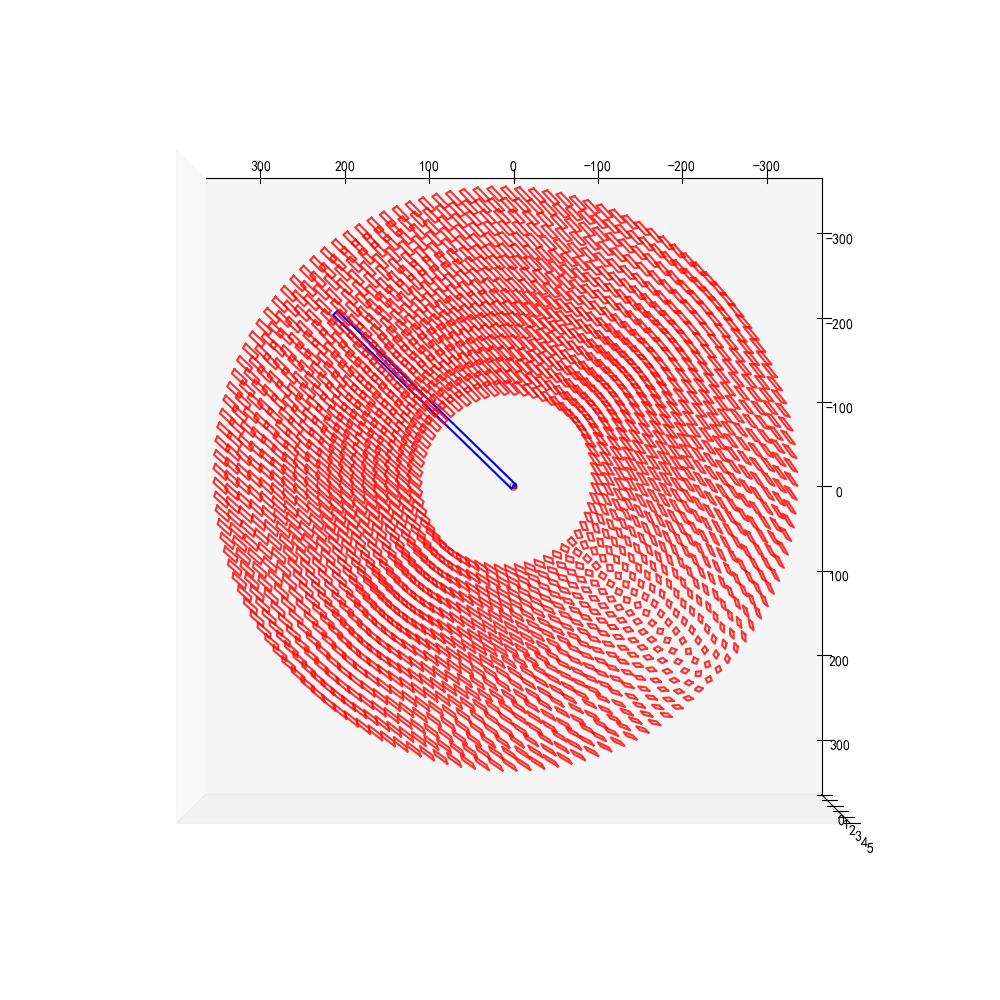
\includegraphics{../A题/head.png}
    }
    \caption{定日镜场可视化图}
    \label{fig:mirror_field}
\end{figure}

\begin{figure}[hptb]
    \centering
    \resizebox{\textwidth}{!}{
        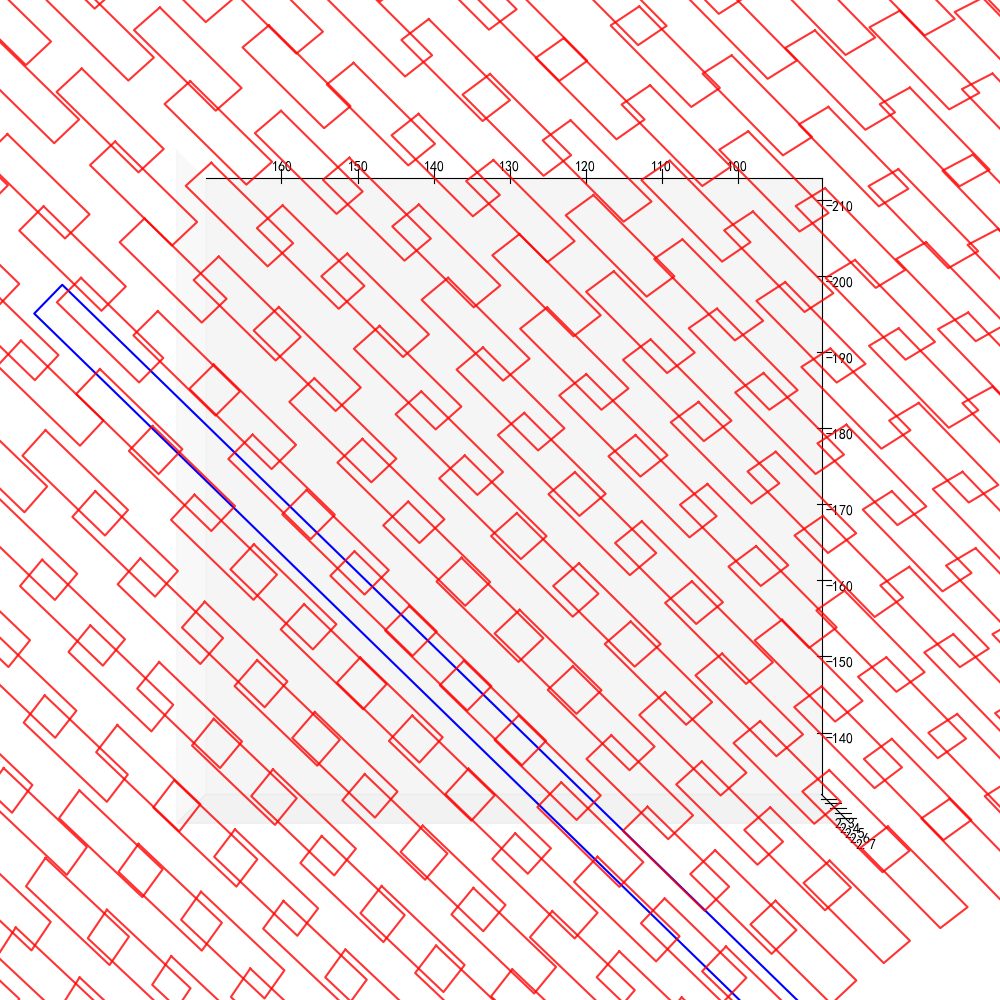
\includegraphics{../A题/detail.png}
    }
    \caption{定日镜场局部可视化图}
    \label{fig:detail}
\end{figure}


% 当太阳光从很远的地方照射过来时,可以将其视作平行光射入定日镜中。图中 a、b 代表太阳入射光线, c 代表 b 入射光线经定日镜反射的光线, 从图 1 中光线路径可见, a 入射光线在入射到 B 镜的过程中恰巧被 A 镜阻挡, 从而使 A 镜在 B 镜上产生了阴影。而 b 光线经由 B 镜反射后的反射光线 c, 其到达吸热器的过程中, 被 B 镜阻挡, 从而产生了 B 镜对 A 镜的挡光现象
% 本文先单独讨论一个定日镜在被太阳照射时其阴影成像情况,设定日镜的四个顶点分别为P1,P2,P3,P4,当太阳光照射到定日镜上时,其影子被投射到地面坐标系上,同理,当考虑到定日镜场所有的镜子时


\textbf{余弦效率(余弦效率理论模型)}\space

在太阳光反射的时候,光线不能百分百的被平面镜接收,定日镜的余弦效率也是影响定日镜光学效率的重要因素,如果入射光线正好和定日镜垂直,则入射光线几乎全部被定日镜吸收,但在实际情况中,入射光线与静镜面之间存在一个角度$\beta$,这就导致光线平行于镜面分量的光线无法被反射,被反射的光线只有垂直镜面分量的部分,垂直镜面分量的光线与入射光线的比值形成的余弦角称为余弦效率,由公式$\eta_{cos}=1-$余弦损失可以计算出余弦效率。

\begin{figure}[hptb]
    \centering

    \begin{tikzpicture}
        \draw[->] (-2,0) -- (2,0);
        \draw[->] (0,-0.5) -- (0,2);

        \draw[-latex] (4/2,3/2) -- (0,0);
        \draw[-latex] (0,0) -- (-4/2,3/2);

        \tdplotdrawarc[->]{(0,0,0)}{0.8}{37}{90}{anchor=south}{$\beta$}

        \draw[thick,-latex] (4/3*2,3/3*2) -- (4/3,3/3);
        \draw[dashed,-latex](4/3*2,3/3*2) -- (4/3,3/3*2);
        \draw[dashed,-latex](4/3*2,3/3*2) -- (4/3*2,3/3);
        \draw[dashed] (4/3,3/3*2) -- (4/3,3/3) -- (4/3*2,3/3);

        \node at (4/3*2,3/3*2) [right,font=\fontsize{6pt}{12pt}\selectfont]{入射向量$\vec{R}$};

        \node at (-4/2,3/2) [right,font=\fontsize{6pt}{12pt}\selectfont]{反射向量$\vec{F}$};

        \node at (4/3,3/3*2) [anchor=south,font=\fontsize{6pt}{12pt}\selectfont]{无效辐射};

        \node at (4/3*2,3/3) [right,font=\fontsize{6pt}{12pt}\selectfont]{有效辐射};

        \node at (0,2) [left,font=\fontsize{6pt}{12pt}] {法线 $\vec{N}$};
    \end{tikzpicture}
    \caption{定日镜遮光模型}
    \label{fig:shadow}
\end{figure}

\textbf{大气透射率} \space 根据公式

\begin{equation}
    \eta_{trunc}=0.99321-0.0001176d_{HR}+1.97x10^{-8}xd^{2}_{HR}
\end{equation}

其中$d_{HR}\leq 1000$,由附件可以计算出各个定日镜中心$(x_{i},y_{i},z_{i})$到集热塔中心$(x_{j},y_{j},z_{j})$的距离。在空间坐标系中计算两点之间的距离公式为

\begin{equation}
    d_{HR}=\sqrt{(x_{i}-x_{j})^2+(y_{i}-x_{j})^2+(z_{i}-z_{j})^2}
\end{equation}

最后计算出每个反射到定日镜光线的大气透射率。

\textbf{集热器截断效率(截断效率理论模型)}\space

\begin{equation}
    F(x,y)=\frac{P_{h}}{2\pi\sigma^2_{HF}}exp(-\frac{(x-x_{t})^2+(y-y_{t})^2}{2\sigma^2_{HF}})
\end{equation}

对于上述公式,其中$P_{h}$为定日镜反射的总功率,为$\sigma^2_{HF}$有效偏差,$(x-x_{t})^2+(y-y_{t})^2$为瞄准点在集热塔接受表面上一点$$P_{h}=I_{D}\cdot A_{m}cosw\cdot f_{at}\cdot \rho$$

对于上述公式中$I_{D}$为法向辐射辐照度,$A_{m}$为定日镜镜面面积,$cosw$是太阳光线与定日镜表面法线夹角的余弦因子,$f_{at}$是大气透射率,$\rho$是定日镜镜面反射率

有效误差是由四个高斯误差函数卷积的结果,由于太阳强度在太阳的圆盘面上的不均匀分布而导致太阳形状误差,由镜面斜率误差引起的光束质量误差,如果入射光线不平行于镜子的法线,则表示反射光线的任何额外变形的像散误差,以及跟踪误差,得到有效误差公式如下:

\begin{equation}
    \sigma_{HF}=\frac{\sqrt{D^{2}(\sigma^2_{sun}+\sigma^2_{bq}+\sigma^2_{ast}+\sigma^2_{t})}}{\sqrt{cos rec}}
\end{equation}

式中$D$为定日镜中心与瞄准点之间的距离,$cos,rec$为定日镜中心与瞄准点之间夹角的余弦值,反射光线与接收表面的法线。光束质量误差是定日镜表面缺陷造成的,与斜面误差的关系如下:
\begin{equation}
    \sigma_{bq}=(2\sigma_{s})^2
\end{equation}

像散误差的标准差为:

\begin{equation}
    \sigma_{ast}=\frac{\sqrt{0.5(H^2_{t}+W^2_{s})}}{4D}
\end{equation}


其中$H_t$和$W_s$分别为切向面和矢状面图像尺寸,分别表示为:
$$H_{t}=d\left|\frac{D}{f}-cosw\right|$$
$$W_{s}=d\left|\frac{D}{f}cosw-1\right|$$

式中,$f$为焦距,$d$为定日镜的一般尺寸。在本文中,$d$等于定日镜面积的平方根。

拦截效率定义为在某一时间点到达接收机表面的反射功率的分数,计算公式如下:

\begin{equation}
    \eta_{int}=\frac{1}{2\pi\sigma^2_{HF}}\int_{x}\int_{y}exp(-\frac{(x-x_{t})^2+(y-y_{t})^2}{2\sigma^2_{HF}})dxdy
\end{equation}

\textbf{镜面反射率} \space 定日镜镜面反射率是指反射镜的反射率以及镜面脏污程度的综合效率,本文根据题干得到镜面反射率的大小为常数$\eta_{ref}$=0.92。

综合上述所求,利用公式

\begin{equation}
    \eta=\eta_{sb}\eta_{cos}\eta_{at}\eta_{trunc}\eta_{ref}
\end{equation}

求得定日镜光学效率记为$\eta_{k}$,则第k个定日镜的年平均光学效率为

\begin{equation}
    \sum^{m}_{j=1}\sum^{n}_{i=1}\frac{\eta_{ij}}{mn}
\end{equation}

$n$为一天中观测的时间点个数,m为一年观测的月数,其中$\eta_{ij}$表示第j月21日的第i个时间点的定日镜光学效率。定日镜场有N个定日镜,则定日镜场的年平均光学效率为

\begin{equation}
    \sum^{N}_{k=1}\sum^{m}_{j=1}\sum^{n}_{i=1}\frac{\eta_{ij}}{mnN}
\end{equation}

\subsubsection{定日镜的热输出功率模型}

定日镜的热输出功率模型由公式决定

\begin{equation}
    E_{field}=DNI\cdot\sum^{N}_{k}A_{k}\eta_{i}
\end{equation}

其中$A_{i}$为第$i$面定日镜的采光面积。DNI为法向直接辐射辐照度,是指地球上垂直于太阳光线的平面单位面积上、单位时间内接收到的太阳辐射能量 ,可由公式近似计算得出:

\begin{equation}
    DNI=G_{0}[a+b exp(-\frac{c}{sin\alpha_{s}})] \end{equation}

\begin{equation}
    a=0.4237-0.00821(6-H)^2
\end{equation}

\begin{equation}
    b=0.5055+0.00595(6.5-H)^2
\end{equation}

\begin{equation}
    c=0.2711+0.01858(2.5-H)^2
\end{equation}

其中$G_{0}$为太阳常数,其取值为1.366kW/$m^2$,H为海拔高度,单位为km。

在计算遮挡效率时,我们已经求出定日镜能够有效反射光线的面积。最后综合求出定日镜的热输出功率。

\subsubsection{问题一求解结果}

问题一求解结果如下表所示。

\begin{table}[hptb]
    \centering
    \caption{问题一每月21日平均光学效率及输出功率}
    \begin{tabular}{@{}cccccc@{}}
        \toprule
        \multicolumn{1}{c}{日期} & \begin{tabular}[]{@{}c@{}}年平均\\ 光学效率\end{tabular} & \begin{tabular}[]{@{}c@{}}年平均\\ 余弦效率\end{tabular} & \begin{tabular}[]{@{}c@{}}年平均阴影\\ 遮挡效率\end{tabular} & \begin{tabular}[]{@{}c@{}}年平均\\ 截断效率\end{tabular} & \multicolumn{1}{l}{\begin{tabular}[]{@{}l@{}}单位面积镜面年平均\\ 输出热功率(kW/m2)\end{tabular}} \\ \midrule
        1月21日                  & 0.640175062                                       & 0.941080171                                       & 0.966900467                                         & 0.791304086                                       & 63.52151                                                                            \\
        2月21日                  & 0.705274359                                       & 0.982838296                                       & 0.993678156                                         & 0.813218745                                       & 59.4609                                                                             \\
        3月21日                  & 0.723165279                                       & 1                                                 & 0.997545034                                         & 0.816383369                                       & 52.95894                                                                            \\
        4月21日                  & 0.707912234                                       & 0.979297788                                       & 0.997346879                                         & 0.816221201                                       & 46.58219                                                                            \\
        5月21日                  & 0.67829731                                        & 0.938528018                                       & 0.997241228                                         & 0.816134737                                       & 42.31599                                                                            \\
        6月21日                  & 0.662206391                                       & 0.917422085                                       & 0.996611307                                         & 0.815619214                                       & 40.67266                                                                            \\
        7月21日                  & 0.67887962                                        & 0.939157714                                       & 0.99733468                                          & 0.816211217                                       & 42.37486                                                                            \\
        8月21日                  & 0.70920086                                        & 0.981097996                                       & 0.997337931                                         & 0.816213878                                       & 46.84839                                                                            \\
        9月21日                  & 0.723105287                                       & 0.999947217                                       & 0.997530158                                         & 0.816371195                                       & 53.30772                                                                            \\
        10月21日                 & 0.698083516                                       & 0.978685176                                       & 0.990674971                                         & 0.810760962                                       & 59.98714                                                                            \\
        11月21日                 & 0.633229349                                       & 0.936675079                                       & 0.963792065                                         & 0.788760192                                       & 63.81266                                                                            \\
        12月21日                 & 0.598264698                                       & 0.917447655                                       & 0.945949107                                         & 0.77415765                                        & 64.43583                                                                            \\ \bottomrule
    \end{tabular}
\end{table}

图\ref{fig:mirror_field}为定日镜场可视化图,其中红色为定日镜,蓝色为集热塔。


\begin{table}[hptb]
    \centering
    \caption{问题一年平均光学效率及输出功率表}
    \begin{tabular}{@{}cccccc@{}}
        \toprule
        \begin{tabular}[]{@{}c@{}}年平均\\ 光学效率\end{tabular} & \begin{tabular}[]{@{}c@{}}年平均\\ 余弦效率\end{tabular} & \begin{tabular}[]{@{}c@{}}年平均阴影\\ 遮挡效率\end{tabular} & \begin{tabular}[]{@{}c@{}}年平均\\ 截断效率\end{tabular} & \begin{tabular}[]{@{}c@{}}年平均输出热\\ 功率(MW)\end{tabular} & \begin{tabular}[]{@{}l@{}}单位面积镜面年平均\\ 输出热功率(kW/m2)\end{tabular} \\\midrule
        0.679816164                                       & 0.959348099                                       & 0.986828499                                         & 0.807613037                                       & 32.45021676                                            & \multicolumn{1}{c}{53.02323}                                    \\\bottomrule
    \end{tabular}
\end{table}


\subsection{问题二:建立定日镜场布局参数,优化镜面输出热功率}

分析问题可知,需要设计吸收塔坐标位置,定日镜 尺寸、安装高度、定日镜数目、定日镜位置单位镜这些参数,使得在满足额定功率一定的条件下,让面积年平均输出热功率尽量大。我们首先对定日镜场进行初始化布局,建立起定日镜场参数之间的联系,对于优化问题,我们可以基于单目标多约束的粒子群优化算法求解出最优解。

\subsubsection{镜场布局模型的建立}

定日镜场的初始布局,本文采用径向交错的辐射网格状圆形布局方式。
相邻定日镜 无 机械 碰 撞 的 最 小 间 距 通过以下方程求出:

\begin{equation}
    DM=DH+SD
\end{equation}
\begin{equation}
    DH=\sqrt{HH^2+WH^2}
\end{equation}

在上述公式 中 :DM 为 特 征长度,表示相邻定日镜间 无 碰 撞 最 小 间 距 ;DH 为定日镜对角线长度; 为定日镜长度;WH 为定日镜宽度;SD 为定日镜间的最小安全距离。

镜场分成 i 个区域,每个区域中各环之间的径向间距相等,镜场径向最小间距出现在靠近中央吸收塔侧的第 1、2 环之间,给出下面公式  :

\begin{equation}
    \Delta R_{min}=DMcos30 degree \\
    \Delta R_{1}=\Delta R_{min} \\
    \Delta R_{2}=x_{i}\Delta R_{min} \\
    \ldots \\
    \Delta R_{i}=x_{i}\Delta R_{min} \\
\end{equation}

在上述公式中:$\Delta R_{min}$为镜场径向最小间距;$\Delta R_{i}$ 为镜场第 i 区域中定日镜相邻环之间的径向间距;$\Delta X_{i}$为径向间距的修正系数,取 $x \geq 1 $。

定日镜的周向间距 $\Delta Az_{i}$ 为镜场第 i 个区域中首环周向相邻定日镜之间的夹角值,可通过下面公式求出:$$\Delta Az_{1}=2acrsin(DM/2R_{min})\approx DM/R_{min} $$

在上述公式中:$R_{min}$ 为镜场正北方向上最小环定日镜与聚光塔底中心的径向间距,即最内环径向半径。
随着镜场环数的增加, 定日镜的周向间距开始发生变化,各区域间的周向间距呈规律减少趋势,由几何法得到  $$\Delta Az_{2}=\Delta Az_{1}/2$$

$$\Delta Az_{i}=\Delta Az_{i-1}/2$$

求镜场各区域对应环上定日镜的数目以及径向半径需要用到以下公式  :

$$N_{helio1,N_{row1}}=N_{helio1,1}=2\pi /\Delta Az_{1}=2\pi R_{min}/DM$$
$$R_{1,1}=R_{min}=N_{helio1,1}DM/2\pi$$
$$R_{1,N_{row1}}=R_{1,1}+(N_{row1-1})\Delta R_min$$

同理有:

$$N_{helio2,N_{row2}}=N_{helio2,1}=4\pi R_{1,1}/DM$$
$$N_{helio3,N_{row3}}=N_{helio3,1}=8\pi R_{1,1}/DM$$
$$\ldots$$
$$N_{helioi,N_{rowi}}=N_{helioi,1}=2^{i}\pi R_{1,1}/DM$$
$$R_{i,1}=2^{i-1}R_{1,1}$$
$$R_{i,N_{rowi}}=2^{i-1}R_{1,1}+(N_{rowi-1})\Delta R_min$$

镜场各分区排布的定日镜环数可通过:

$$N_{row1}=\frac{(R_{2,1}-R{1,1})}{\Delta R_{min}}=round(2^0(R_{1,1}/\Delta R_{min}))$$
$$N_{row2}=round(2^1(R_{1,1}/\Delta R_{min}))$$
$$N_{rowi}=round(2^{i-1}(R_{1,1}/\Delta R_{min}))$$

$N_{row}$为镜场第 1 区域的环数;$N_{rowi}$ 为镜场第 i 区域的环数:$R_{1,1}$为镜场第 1 区域首环半径;$R_{i,row1}$为镜场第 1 区域末环半径;$R_{1,rowi}$ 为镜场第 i 区域首环半径;$R_{i,rowi}$为镜场第 i区域末环半径。

\begin{figure}[hptb]
    \centering

    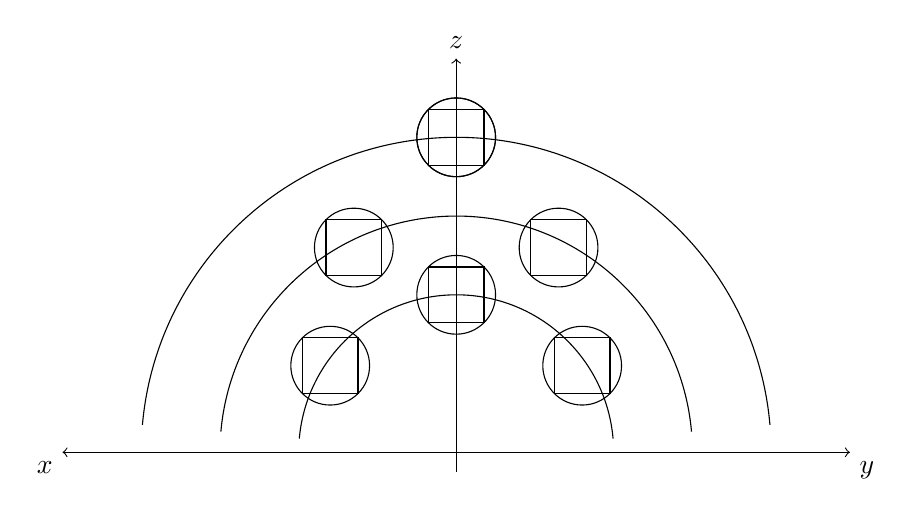
\begin{tikzpicture}
        \draw[->] (0,0) -- (-5,0) node[anchor=north east]{$x$};
        \draw[->] (0,0) -- (5,0) node[anchor=north west]{$y$};
        \draw[->] (0,-0.25) -- (0,5) node[anchor=south]{$z$};

        \tdplotdrawarc[]{(0,0,0)}{2}{5}{175}{anchor=north}{}
        \tdplotdrawarc[]{(0,0,0)}{3}{5}{175}{anchor=north}{}
        \tdplotdrawarc[]{(0,0,0)}{4}{5}{175}{anchor=north}{}

        \begin{scope}
            \newcommand{\cx}{0};
            \newcommand{\cy}{2};

            \draw (\cx,\cy) circle (0.5);
            \draw (\cx + 0.353553391, \cy + 0.353553391) -- (\cx - 0.353553391,\cy + 0.353553391) --  (\cx - 0.353553391,\cy - 0.353553391) -- (\cx + 0.353553391, \cy - 0.353553391) -- cycle;
        \end{scope}

        \begin{scope}
            \newcommand{\cx}{0};
            \newcommand{\cy}{4};

            \draw (\cx,\cy) circle (0.5);
            \draw (\cx + 0.353553391, \cy + 0.353553391) -- (\cx - 0.353553391,\cy + 0.353553391) --  (\cx - 0.353553391,\cy - 0.353553391) -- (\cx + 0.353553391, \cy - 0.353553391) -- cycle;
        \end{scope}

        \begin{scope}
            \newcommand{\cx}{0};
            \newcommand{\cy}{4};

            \draw (\cx,\cy) circle (0.5);
            \draw (\cx + 0.353553391, \cy + 0.353553391) -- (\cx - 0.353553391,\cy + 0.353553391) --  (\cx - 0.353553391,\cy - 0.353553391) -- (\cx + 0.353553391, \cy - 0.353553391) -- cycle;
        \end{scope}

        \begin{scope}
            \newcommand{\cx}{1.3};
            \newcommand{\cy}{2.6};

            \draw (\cx,\cy) circle (0.5);
            \draw (\cx + 0.353553391, \cy + 0.353553391) -- (\cx - 0.353553391,\cy + 0.353553391) --  (\cx - 0.353553391,\cy - 0.353553391) -- (\cx + 0.353553391, \cy - 0.353553391) -- cycle;
        \end{scope}

        \begin{scope}
            \newcommand{\cx}{1.6};
            \newcommand{\cy}{1.1};

            \draw (\cx,\cy) circle (0.5);
            \draw (\cx + 0.353553391, \cy + 0.353553391) -- (\cx - 0.353553391,\cy + 0.353553391) --  (\cx - 0.353553391,\cy - 0.353553391) -- (\cx + 0.353553391, \cy - 0.353553391) -- cycle;
        \end{scope}

        \begin{scope}
            \newcommand{\cx}{-1.3};
            \newcommand{\cy}{2.6};

            \draw (\cx,\cy) circle (0.5);
            \draw (\cx + 0.353553391, \cy + 0.353553391) -- (\cx - 0.353553391,\cy + 0.353553391) --  (\cx - 0.353553391,\cy - 0.353553391) -- (\cx + 0.353553391, \cy - 0.353553391) -- cycle;
        \end{scope}

        \begin{scope}
            \newcommand{\cx}{-1.6};
            \newcommand{\cy}{1.1};

            \draw (\cx,\cy) circle (0.5);
            \draw (\cx + 0.353553391, \cy + 0.353553391) -- (\cx - 0.353553391,\cy + 0.353553391) --  (\cx - 0.353553391,\cy - 0.353553391) -- (\cx + 0.353553391, \cy - 0.353553391) -- cycle;
        \end{scope}
    \end{tikzpicture}
    \caption{镜场布局模型}
    \label{fig:mirror_field}
\end{figure}

\begin{figure}[htbp]
    \centering
    \resizebox{\textwidth}{!}{
        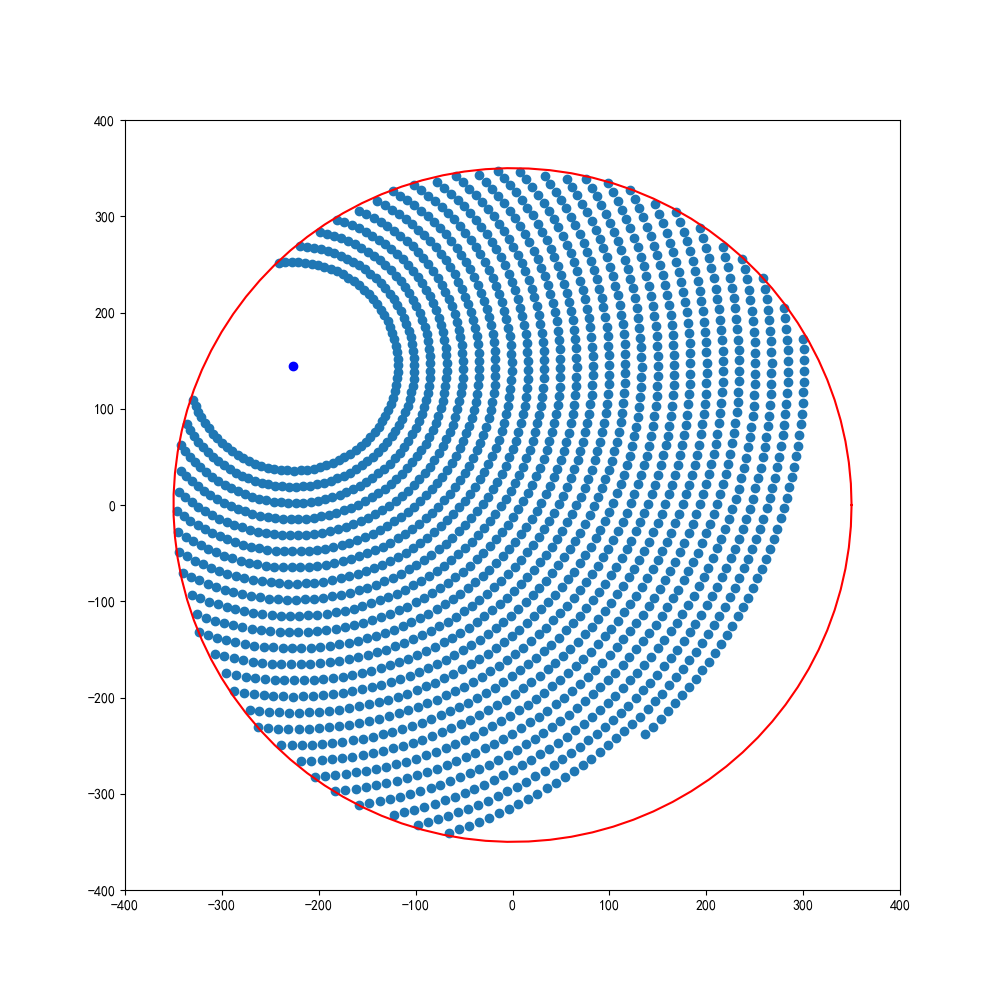
\includegraphics{../A题/full.png}
    }
    \label{fig:full}
\end{figure}

\subsubsection{粒子群优化(Particle Swarm Optimization)算法}

粒子群优化算法是一种计算方法,它受到了鸟群或鱼群等生物群体行为的启发。PSO用于解决各种优化问题,尤其是在搜索空间复杂或庞大的情况下。PSO的基本思想是模拟个体粒子在多维搜索空间中的移动,以寻找近似最优解。每个粒子表示潜在解决方案,它根据其位置和速度以及与其他粒子的互动来更新自己的位置和速度。这个过程一直持续,直到找到满意的解或达到了指定的停止条件。总之,PSO是一种寻找最优解的算法,通过模拟粒子的行为来不断改进解的质量。

假设$X_{i}=(x_{i,1},x_{i,2},\ldots,x_{i,n})$是微粒$i$的当前位置,$V_{i}=(y_{i,1},y_{i,2},\ldots,y_{i,n})$是微粒$i$的当前飞行速度,那么,基本粒子群优化算法的进化方程为:$$v_{i,j}(t+1)=v_{i,j}(t)+c_{1}rand_{1}()(p_{i,j}(t)-x_{i,j}(t))+c_{2}rand_{2}()(p_{g,j}(t)-x_{i,j}(t))$$

$$x_{i,j}(t+1)=x_{i,j}(t)+v_{i,j}(t+1)$$
$$P_{i}(t)=(p_{i,1}(t),p_{i,2}(t),\ldots,p_{i,n}(t),)$$
$$P_{g}(t)=(p_{g,1}(t),p_{g,2}(t),\ldots,p_{g,n}(t),)$$

在上述式子中,t表示迭代代数;$P_{i}(t)$表示微粒$i$迄今为止达到过的最好位置;$P_{g}(t)$是当前粒子群搜索到的最好位置,$c_{1}$、$c_{2}$分别为认知学习因子和社会学系因子,通常在0-2间取值。$rand_1()$、$rand_2()$是在[0,1]上的两个相互独立的随机数

其实现步骤如下:

第一步:在允许的范围内,初始化搜索点的位置及其速度,每个粒子的坐标设置为其当前位置,且计算出其相应的个体极值(即个体极值点的适应度值),而全局极值(即全局极值点的适应度值)就是个体极值中最好的,记录该最优值的粒子序号,并将 $P_{g}(t)$设置为该最优粒子的当前位置;

第二步: 计算粒子的适应度值,即目标函数值,如果优于该粒子当前的个体极值,则将 $P_{i}(t)$设置为该粒子的位置,且更新个体极值。如果所有粒子的个体极值中最好的好于当前的全局极值,则将 $P_{g}(t)$设置为该粒子的位置,记录该粒子的序号,且更新全局极值;

第三步:通过PSO的计算公式,对每一个粒子的速度和位置进行更新;

第四步: 检验是否符合结束条件,若当前的迭代次数达到了预先设定的最大次数(或达到最小错误要求等),则停止迭代,输出最优解  ,若不满足条件则重新进入循环再次计算。

\subsubsection{问题二求解结果}

问题二求解结果如下表所示。

\begin{table}[]
    \centering
    \caption{问题二求解结果}
    \begin{tabular}{@{}ccccc@{}}
        \toprule
        吸收塔位置坐标      & 定日镜尺寸(宽x高)         & 定日镜安装高度(m) & 定日镜总面数 & 定日镜总面积(m2)    \\ \midrule
        268.55513007 & 2.5753146x6.020637 & 5.92792577 & 1940   & 30079.7666727 \\ \bottomrule
    \end{tabular}
\end{table}

\subsection{问题三:建立PSO-GA遗传算法,确定最优的布局与参数}

为进一步优化定日镜场的参数,本文建立了PSO-GA算法,采用遗传算法结合粒子群优化算法进行求解。

遗传算法(GA)是一种基于自然选择原理和自然遗传机制的搜索算法,它模拟了生物进化的过程,以实现人工系统中的目标优化。该算法通过群体搜索技术,根据适者生存的原则逐代进化,最终获得最优或接近最优解。其核心操作包括以下步骤:首先生成初始群体,然后评估每个个体的适应度。接着根据适者生存的原则选择出表现良好的个体,再将这些选出的个体进行两两配对,通过随机交叉其染色体的基因以及随机变异某些染色体的基因,从而生成下一代群体。通过不断重复这个过程,使群体逐代演化,直至达到进化终止条件为止。这一过程充分利用了生物进化的概念,用于寻找问题的最佳解或接近最佳解。

\begin{figure}[hptb]
    \centering

    \begin{tikzpicture}[node distance=10pt]
        \node[draw, rounded corners]                        (start)   {开始};
        \node[draw, below=of start]                         (step 1)  {确定可行解域名};
        \node[draw, below=of step 1]                        (step 2)  {进行编码};
        \node[draw, below=of step 2]                        (step 3)  {初始化群体 $P(t)$};
        \node[draw, below=of step 3]                        (step 4)  {评价群体};
        \node[draw, diamond, aspect=2, below=20pt of step 4]     (choice)  {满足终止条件?};
        \node[draw, rounded corners, below=20pt of choice]  (end)     {结束};
        \node[draw, right=20pt of choice]                        (step 5)  {选择 交叉 变异};
        \node[draw, above= of step 5]                       (step 6)  {评价群体};
        \node[draw, above= of step 6]                   (step 7)  {产生新一代群体};

        \draw[->] (start)  -- (step 1);
        \draw[->] (step 1) -- (step 2);
        \draw[->] (step 2) -- (step 3);
        \draw[->] (step 3) -- (step 4);
        \draw[->] (step 4) -- (choice);
        \draw[->] (choice) -- node[left]  {是} (end);
        \draw[->] (choice) -- node[above] {否}  (step 5);
        \draw[->] (step 5) -- (step 6);
        \draw[->] (step 6) -- (step 7);
        \draw[->] (step 7) -- (step 4);
    \end{tikzpicture}

    \caption{PSO的基本流程}
    \label{fig:pso}
\end{figure}

具体实现步骤如下:

第一步:确定遗传算法中相应的参数,如种群规模 M ,变异概率 pm ,交叉概率pc ,进化代数阈值iter 等;

第二步:随机生成初始种群,即初始化种群;

第三步:计算目标函数值以评价群体;

第四步:若满足停止条件,则算法结束,否则进入第五步

第五步:进行遗传操作,即选择,交叉,变异,生成新一代群体,再继续进入第三步进一步优化

本文中引入了PSO-GA混合算法,这种算法以 粒子群优化算法 和 遗传算法 两种算法作为求解模型的基础,充分的结合了两者的优点,与此同时又减少了部分算法存在的缺陷,在优化方程系数方面有更好地表现。

在 混合算法中目前的研究和使用上,目标值受相关因素的影响可分别建立为线性、指数型、二次型三种模型,其表达式分别如下:

$$Q_{1}=\sum^{N}_{i=1}\tau_{i} F_{i}+\tau_{0}$$
$$Q_{2}=\sum^{N}_{i=1}\tau_{i} F^{\tau_{i}}_{i}+\tau_{0}$$
$$Q_{3}=\sum^{N}_{i=1}\tau_{i}F_{i}+\tau_{0}+\sum^{N}_{i=1}\sum^{N}_{j=i+1}k_{ij}F_{i}F_{j}+\sum^{N}_{I=1}u_{i}F^2_{i}$$

其中$F_{i}$为第$i$个影响因素,$\tau_{0}$,$\tau_{i}$,$k_{ij}$和$u_{i}$为系数,$N$为影响因素个数。实际操作中,具体流程如图。

\begin{figure}[hptb]
    \centering

    \begin{tikzpicture}
        \node[draw] (box 0) {$p_{0}$};
        \node[draw, right=of box 0] (box 1) {$p_{1}$};
        \node[right=of box 1] (box 3) {$\dots$};
        \node[draw, right=of box 3] (box 4) {$p_{i}$};
        \node[draw, right=of box 4] (box 5) {$p_{i+1}$};

        \node[draw, below=20pt of box 3] (box 6) {PSO 演变};
        \node[draw, below=10pt of box 6] (box 7) {最适值排序};

        \node[below=50pt of box 7] (box 8) {$\dots$};
        \node[draw, left=of box 8] (box 9) {$q_{1}$};
        \node[draw, left=of box 9] (box 10) {$q_{0}$};
        \node[draw, right=of box 8] (box 11) {$q_{i}$};
        \node[draw, right=of box 11] (box 12) {$q_{i+1}$};

        \node[above=5pt of box 9] (box 13) {最好};
        \node[above=5pt of box 11] (box 14) {最差};

        \node[draw, below=30pt of box 9] (box 15) {更新速度};
        \node[draw, below=24pt of box 15] (box 16) {更新位置};

        \node[draw, below=30pt of box 11] (box 17) {选择};
        \node[draw, below=4pt of box 17] (box 18) {交叉};
        \node[draw, below=4pt of box 18] (box 19) {变异};


        \node[below=200pt of box 7] (box 20) {$\dots$};
        \node[draw, left=of box 20] (box 21) {$q_{1}$};
        \node[draw, left=of box 21] (box 22) {$q_{0}$};
        \node[draw, right=of box 20] (box 23) {$q_{i}$};
        \node[draw, right=of box 23] (box 24) {$q_{i+1}$};

        \node[below=5pt of box 21] (box 25) {最好};
        \node[below=5pt of box 23] (box 26) {最差};

        \foreach \i in {0, 1, 3, 4, 5}
        \draw[->] (box \i)  -- (box 6);
        \draw[->] (box 6)  -- (box 7);
        \draw[->] (box 7)  -- (box 8);

        \foreach \i in {8,9,...,12}
        \draw[->] (box 8)  -- (box 15) node[midway,above] {保留};

        \draw[->] (box 8)  -- (box 17) node[midway,above] {舍弃};
        \draw[->] (box 15)  -- (box 16);
        \draw[->] (box 16)  -- (box 20);
        \draw[->] (box 17)  -- (box 18);
        \draw[->] (box 18)  -- (box 19);
        \draw[->] (box 19)  -- (box 20);

        \node[below=80pt of box 20] (temp){};
        \node[right=150pt of temp] (temp1){};
        \node[above=295pt of temp1] (temp2){};

        \draw[] (box 20) -- (temp) -- (temp1) -- (temp2) -> (box 7);

    \end{tikzpicture}
    \caption{PSO-GA混合算法流程图}
    \label{fig:pso-ga}
\end{figure}

该混合算法的具体实现步骤如下:

第一步:确定相关系数,如粒子种群规模 M ,由 PSO 演变后保留的粒子规模 M' ,PSO 认知学习因子和社会学系因子 c1 及 c2 , GA 的交叉以及突变概率 pc 和 pm ,粒子最大速度vimax , 粒子群优化算法迭代代数阈值iter1和 混合算法迭代代数阈值iter2 ;

第二步:实际编码确定式由粒子群优化算法的编码形式的系数决定

第三步:若 混合算法 迭代达到iter2 ,则算法结束,输出最优适应度、最优位置解。若未得到最优解则进入第四步

第四步:若 粒子群优化算法的迭代达到iter1,则算法结束,否则继续进入第五步

第五步:类似 粒子群优化算法,根据下式,更新离子的速度和位置;

$$v^{t+1}_{id}=\chi\cdot[v^{t}_{id}+c_{1}rand_{1}()P^{t}_{id}-x^{t}_{id}]$$

\begin{figure}
    \centering
    \resizebox{\textwidth}{!}{
        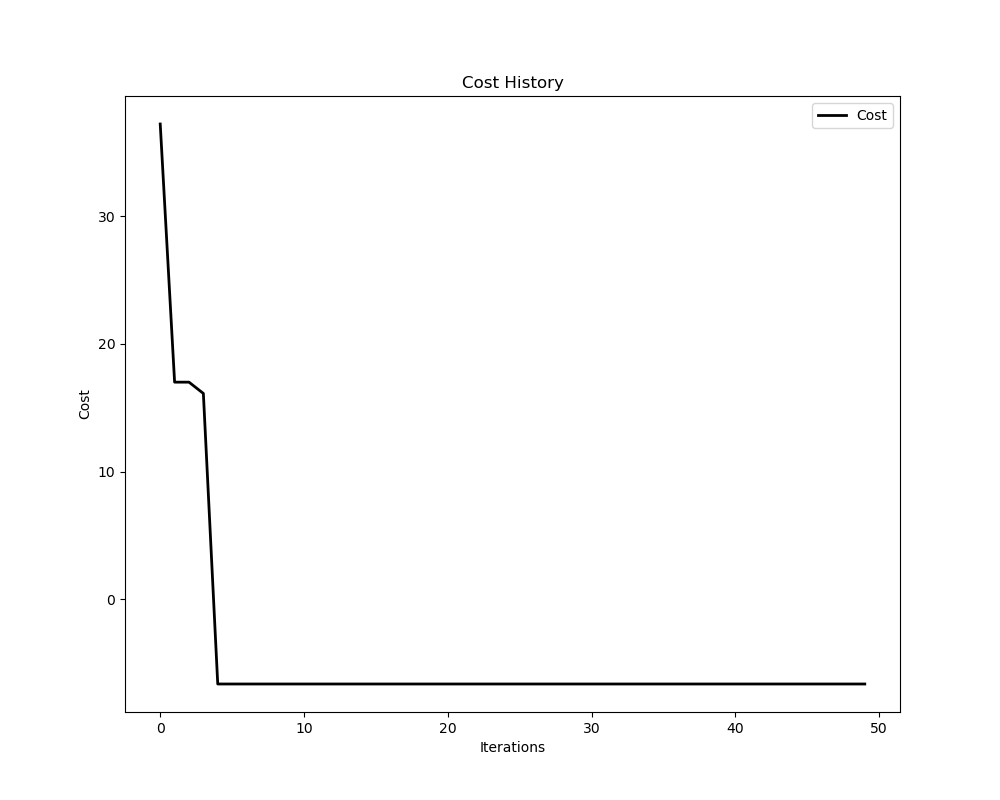
\includegraphics{../A题/cost_history.png}
    }
    \caption{PSO-GA算法收敛曲线}
\end{figure}

上图为PSO-GA算法收敛曲线,可以看出,PSO-GA算法在迭代次数达到10次时,已经收敛到最优解。


\section{模型的评价}

\subsection{模型优点}

\subsection{模型不足}



\bibliographystyle{gbt7714-numerical}
\bibliography{bib}


\newpage
%附录
\begin{appendices}

    \section{问题一模型求解 Python代码}


    \begin{lstlisting}[language=python]
    import datetime

    import geopandas
    import numpy
    import pandas
    import tqdm
    from matplotlib import pyplot as plt
    from shapely import Polygon
    from tqdm.contrib.concurrent import process_map
    
    phi = numpy.radians(39.4)
    
    
    def rotate_x(v, theta):
        """
        绕x轴旋转
        :param v:
        :param theta:
        :return:
        """
        return numpy.array(
            [
                v[0],
                v[1] * numpy.cos(theta) - v[2] * numpy.sin(theta),
                v[1] * numpy.sin(theta) + v[2] * numpy.cos(theta),
            ]
        )
    
    
    def rotate_y(v, theta):
        """
        绕y轴旋转
        :param v:
        :param theta:
        :return:
        """
        return numpy.array(
            [
                v[0] * numpy.cos(theta) + v[2] * numpy.sin(theta),
                v[1],
                -v[0] * numpy.sin(theta) + v[2] * numpy.cos(theta),
            ]
        )
    
    
    def rotate_z(v, theta):
        """
        绕z轴旋转
        :param v:
        :param theta:
        :return:
        """
        return numpy.array(
            [
                v[0] * numpy.cos(theta) - v[1] * numpy.sin(theta),
                v[0] * numpy.sin(theta) + v[1] * numpy.cos(theta),
                v[2],
            ]
        )
    
    
    class Sun:
        G = 1.366  # 太阳常数
    
        def __init__(self, time):
            self.time = time
    
            self.delta = self._delta()
            self.omega = self._omega()
            self.alpha = self._alpha()
            self.gamma = self._gamma()
            self.theta = self._theta()
            self.dni = self._dni()
    
            self.n = self._n()
    
        def __repr__(self):
            return f"<Sun time={self.time}>"
    
        def _alpha(self):
            return numpy.arcsin(
                numpy.clip(
                    numpy.cos(self.delta) * numpy.cos(phi) * numpy.cos(self.omega)
                    + numpy.sin(self.delta) * numpy.sin(phi),
                    -1,
                    1,
                )
            )
            pass
    
        def _gamma(self):
            return numpy.arccos(
                numpy.clip(
                    (numpy.sin(self.delta) - numpy.sin(self.alpha) * numpy.sin(phi))
                    / (numpy.cos(self.alpha) * numpy.cos(phi)),
                    -1,
                    1,
                )
            )
    
        def _omega(self):
            return numpy.pi / 12 * (self.time.hour + self.time.minute / 60 - 12)
    
        def _delta(self):
            d = (self.time - datetime.datetime(self.time.year, 3, 21)).days
            day = (d + 365) % 365
            return numpy.arcsin(
                numpy.clip(
                    numpy.sin(2 * numpy.pi * day / 365)
                    * numpy.sin(2 * numpy.pi * 23.45 / 360),
                    -1,
                    1,
                )
            )
    
        def _theta(self):
            return numpy.pi / 2 - self.alpha
    
        def _dni(self):
            a = 0.34981
            b = 0.5783875
            c = 0.275745
            return self.G * (a + b * numpy.exp(-c / numpy.sin(self.alpha)))
    
        def _n(self):
            return -numpy.array(
                [
                    numpy.cos(self.alpha) * numpy.cos(self.gamma),
                    numpy.cos(self.alpha) * numpy.sin(self.gamma),
                    numpy.sin(self.alpha),
                ]
            )
    
    
    class Tower:
        def __init__(self, sun: Sun, x=0, y=0, z=80, h=8, r=3.5):
            self.sun = sun
    
            self.x = x
            self.y = y
            self.z = z
    
            self.coordinate = numpy.array([x, y, z])
    
            self.h = h
            self.r = r
    
            self.center = numpy.array([x, y, 0])
    
            self.vertex = self._vertex()
            self.project = self._project()
    
        @property
        def vertex_area(self):
            return Polygon(self.vertex).area
    
        def _vertex(self):
            # 变换后的宽高
            h = (self.z + self.h / 2) / numpy.cos(self.sun.alpha)
            w = self.r * 2
    
            x = [1, -self.sun.n[0] / self.sun.n[1], 0]
            x = x / numpy.linalg.norm(x)
            y = numpy.cross(self.sun.n, x)
    
            # 底边中心 为原点
            left_down = -0.5 * w * x
            left_up = 0.5 * w * x
            right_up = 1 * h * y + 0.5 * w * x
            right_down = 1 * h * y - 0.5 * w * x
    
            return numpy.array([left_down, left_up, right_up, right_down])
    
        def _project(self):
            ans = numpy.array(
                [point + (-point[2] / self.sun.n[2] * self.sun.n) for point in self.vertex]
            )
            # z = 0
            ans[:, 2] = 0
            return ans
    
        def __repr__(self):
            return f"<Tower x={self.x}, y={self.y}, z={self.z}>"
    
    
    class Mirror:
        def __init__(
            self,
            tower: Tower,
            x: float = 0,
            y: float = 0,
            z: float = 4,
            h: float = 6,
            w: float = 6,
        ):
            self.tower = tower
    
            self.x = x
            self.y = y
            self.z = z
    
            self.coordinate = numpy.array([x, y, z])
    
            self.h = h
            self.w = w
            self.r = numpy.sqrt(h**2 + w**2) / 2
    
            self.v_tower = self._v_tower()
            self.n_tower = self._n_tower()
    
            self.n = self._n()  # 平面法向量
    
            self.vertex = self._vertex()
            self.project = self._project()
    
            self.area = 0
    
        def _v_tower(self):
            return self.tower.coordinate - self.coordinate
    
        def _n_tower(self):
            return self.v_tower / numpy.linalg.norm(self.v_tower)
    
        def _n(self):
            v = self.n_tower - self.tower.sun.n
            return v / numpy.linalg.norm(v)
    
        def _vertex(self):
            x = [1, -self.n[0] / self.n[1], 0]
            x = x / numpy.linalg.norm(x)
            y = numpy.cross(self.n, x)
    
            left_down = self.coordinate - 0.5 * self.h * y - 0.5 * self.w * x
            left_up = self.coordinate - 0.5 * self.h * y + 0.5 * self.w * x
            right_up = self.coordinate + 0.5 * self.h * y + 0.5 * self.w * x
            right_down = self.coordinate + 0.5 * self.h * y - 0.5 * self.w * x
    
            return numpy.array([left_down, left_up, right_up, right_down])
    
        def _project(self):
            ans = numpy.array(
                [
                    point + (-point[2] / self.tower.sun.n[2] * self.tower.sun.n)
                    for point in self.vertex
                ]
            )
            # z = 0
            ans[:, 2] = 0
            return ans
    
        def __repr__(self):
            return f"<Mirror x={self.x}, y={self.y}, z={self.z}>"
    
    
    def get_shadow_efficiency(tower, mirror_list):
        geo = [Polygon(i.project) for i in mirror_list]
        geo.append(Polygon(tower.project))
    
        gdf = geopandas.GeoDataFrame(geometry=geo)
    
        area = gdf.area.sum()
    
        intersection = gdf.unary_union.intersection(gdf.unary_union)
        overlap = intersection.area
    
        # 重复部分
        return numpy.array([overlap / area] * len(mirror_list))
    
    
    def get_cosine_efficiency(sun, mirror_list):
        return numpy.clip(numpy.cos(sun.delta), -1, 1).repeat(len(mirror_list))
    
    
    def get_atmosphere_efficiency(tower: object, mirror_list: object) -> numpy.array:
        coordinate = tower.coordinate
        distance = numpy.array(
            [numpy.linalg.norm(mirror.coordinate - coordinate) for mirror in mirror_list]
        )
        return numpy.array(
            [0.99321 - 0.0001176 * d + 1.97 * 1e-8 * numpy.power(d, 2) for d in distance]
        )
    
    
    def get_truncation_efficiency(tower, mirror_list, shadow_efficiency):
        dat = []
        for index, mirror in enumerate(mirror_list):
            dis = mirror.h / numpy.sin(4.65 * 10**-3)
            d = numpy.linalg.norm(mirror.coordinate[:2] - tower.coordinate[:2])
            ratio = (dis + d) / dis
    
            mirror_area = mirror.w * mirror.w * ratio
            theta = mirror.v_tower[2] / numpy.linalg.norm(mirror.v_tower[:2])
    
            head_area = tower.r * 2 * tower.h * numpy.cos(theta)
            dat.append(mirror_area / head_area * shadow_efficiency[index])
        return numpy.array(dat)
    
    
    def get_output_heat_power(sun, tower, mirror_list, optical_efficiency):
        return sun.dni * numpy.sum(
            [mirror.area * optical_efficiency[i] for i, mirror in enumerate(mirror_list)]
        )
    
    
    def compute(sun, tower, mirror_list):
        init_mirror_area(tower, mirror_list)
    
        shadow_efficiency = get_shadow_efficiency(tower, mirror_list)
        cos_efficiency = get_cosine_efficiency(sun, mirror_list)
        atmosphere_efficiency = get_atmosphere_efficiency(tower, mirror_list)
        truncation_efficiency = get_truncation_efficiency(
            tower, mirror_list, shadow_efficiency
        )
        optical_efficiency = (
            shadow_efficiency
            * cos_efficiency
            * atmosphere_efficiency
            * truncation_efficiency
            * 0.92
        )
    
        output_heat_power = get_output_heat_power(
            sun, tower, mirror_list, optical_efficiency
        )
    
        return numpy.array(
            [
                sun.time,
                numpy.mean(optical_efficiency),
                numpy.mean(cos_efficiency),
                numpy.mean(shadow_efficiency),
                numpy.mean(truncation_efficiency),
                output_heat_power,
            ]
        )
    
    
    def init_mirror_area(tower, mirrors):
        poly = [Polygon(mirror.project) for mirror in mirrors]
        poly.append(Polygon(tower.project))
    
        last = 0
        for i in range(1, len(poly)):
            a = geopandas.GeoDataFrame(geometry=poly[:i]).area.sum() - last
            last += a
            mirrors[i - 1].area = a
    
    
    def main():
        date = get_all_time()
    
        sun = [Sun(time) for time in date]
        tower = [Tower(s) for s in sun]
        mirror_list = [[Mirror(t, x[i], y[i]) for i in range(len(x))] for t in tower]
    
        data = process_map(compute, sun, tower, mirror_list, chunksize=1)
        # data = [compute(i) for i in tqdm.tqdm(date)]
    
        pd = pandas.DataFrame(
            columns=["日期", "平均光学效率", "平均余弦效率", "平均遮挡效率", "平均截断效率", "单位面积镜面年平均输出热功率"]
        )
    
        for i in data:
            pd.loc[len(pd)] = i
    
        pd.to_excel("result.xlsx", index=False)
    
    
    def get_all_time():
        date = []
        for month in range(1, 13):
            for hour, minute in [(9, 0), (10, 30), (12, 0), (13, 30), (15, 0)]:
                date.append(datetime.datetime(2023, month, 21, hour, minute))
        return date
    
    
    def draw():
        date = []
        for month in range(1, 13):
            for hour, minute in [(9, 0), (10, 30), (12, 0), (13, 30), (15, 0)]:
                date.append(datetime.datetime(2023, month, 21, hour, minute))
    
        for index, time in enumerate(tqdm.tqdm(date[::])):
            sun = Sun(time)
            tower = Tower(sun)
            mirror_list = [Mirror(tower, x[i], y[i]) for i in range(len(x))]
    
            fig = plt.figure(figsize=(25, 25))
            ax = fig.add_subplot(111, projection="3d")
    
            ax.plot(0, 0, 0, ".", color="r")
    
            # ax.plot(*tower.coordinate, "o", color="b")
    
            # 圆柱
            theta = numpy.linspace(0, 2 * numpy.pi, 1000)
            z_ = numpy.linspace(0, 20, 1000)
            z_ = numpy.linspace(0, 20, 1000)
            theta, z_ = numpy.meshgrid(theta, z_)
            x_ = tower.r * numpy.cos(theta)
            y_ = tower.r * numpy.sin(theta)
            ax.plot_surface(x_, y_, z_, alpha=0.4)
    
            v = numpy.array([*tower.project, tower.project[0]])
            ax.plot(v.T[0], v.T[1], v.T[2], color="b")
            # v = numpy.array([*tower.vertex, tower.vertex[0]])
            # ax.plot(v.T[0], v.T[1], v.T[2], color="g")
    
            for mirror in mirror_list[::]:
                v = numpy.array([*mirror.project, mirror.project[0]])
                ax.plot(v.T[0], v.T[1], v.T[2], color="r", alpha=0.8)
                # ax.plot(
                #     *mirror.coordinate,
                #     ".",
                # )
    
            # z轴尺寸
            ax.set_zlim(0, 5)
    
            # 锁定视角
            ax.view_init(azim=90, elev=90)
    
            # 减小空白
            plt.subplots_adjust(left=0, right=1, bottom=0, top=1)
    
            plt.savefig(f"img/{index}.png")
            # plt.show()
            plt.close()
            pass
    
    
    if __name__ == "__main__":
        data = pandas.read_excel("附件.xlsx")
        x = data["x坐标 (m)"]
        y = data["y坐标 (m)"]
    
        main()
        # draw()
        pass
    
\end{lstlisting}

    \section{问题二与问题三模型求解 Python代码}

    \begin{lstlisting}[language=python]
    # Particle swarm optimization algorithm
    import datetime
    
    import numpy
    import pandas as pd
    import pyswarms
    from matplotlib import pyplot as plt
    from pyswarms.utils.plotters import plot_cost_history
    from tqdm.contrib.concurrent import process_map
    
    from A import (
        Mirror,
        rotate_z,
        compute,
        Sun,
        Tower,
        get_all_time,
    )
    
    
    def arrangement(
        sun,
        tower,
        z,
        w,
        n,
    ):
        """
        定日镜的排列
        :param sun: 太阳
        :param tower: 吸收塔
        :param z: 定日镜的安装高度
        :param w: 定日镜的尺寸
        :param n: 定日镜的数目
    
        """
        center = numpy.array([tower.x, tower.y, 0])
    
        cnt = 0
        lap = 0
    
        space = 2.5
        h = z if z > w / 2 else w / 2
        r = (w / 2) * numpy.sqrt(2)
    
        mirror_list = []
        while cnt < n:
            delta = 100 + r + lap * r * 2
            theta = numpy.sin((r + space) / (r + delta))
            v = rotate_z(numpy.array([0, delta + r + lap * r * 2, h]), sun.theta)
            for rad in numpy.linspace(
                (lap % 2) * theta, numpy.pi * 2, int(numpy.pi * 2 // theta)
            ):
                location = center + rotate_z(v, numpy.pi * 2 - rad)
                if numpy.linalg.norm(location[:2]) > 350:
                    continue
                mirror_list.append(Mirror(tower, *location, w, w))
                cnt += 1
                if cnt >= n:
                    break
            lap += 1
    
        return mirror_list
    
        # plt.figure(figsize=(20, 20))
        #
        # # circle
        # # theta = numpy.linspace(0, 2 * numpy.pi, 100)
        # # x = 350 * numpy.cos(theta)
        # # y = 350 * numpy.sin(theta)
        # # plt.plot(x, y, color="r")
        # # plt.plot(0.0, 0.0, "o", color="r")
        # # plt.xlim(-400, 400)
        # # plt.ylim(-400, 400)
        #
        # plt.scatter([i.x for i in mirror_list], [i.y for i in mirror_list])
        # plt.plot(*center[:2], "o", color="r")
        # plt.savefig("full.png")
        # plt.show()
        # return mirror_list
    
    
    # def compute(args):
    #     """
    #     :param time: 时间
    #     :param r: 吸收塔的 r 半径
    #     :param t: 吸收塔的 θ 角度
    #     :param z: 定日镜的安装高度
    #     :param w: 定日镜的尺寸
    #     :param n: 定日镜的数目
    #     :return:
    #     """
    #     (
    #         time,
    #         r,
    #         t,
    #         z,
    #         w,
    #         n,
    #     ) = args
    #     n = int(n)
    #
    #     sun = Sun(time)
    #     tower = Tower(sun, r * numpy.cos(t), r * numpy.sin(t))
    #     mirror_list = arrangement(sun, tower, z, w, n)
    #
    #     init_mirror_area(tower, mirror_list)
    #
    #     shadow_efficiency = get_shadow_efficiency(tower, mirror_list)
    #     cos_efficiency = get_cosine_efficiency(sun, mirror_list)
    #     atmosphere_efficiency = get_atmosphere_efficiency(tower, mirror_list)
    #     truncation_efficiency = get_truncation_efficiency(
    #         tower, mirror_list, shadow_efficiency
    #     )
    #     optical_efficiency = (
    #         shadow_efficiency
    #         * cos_efficiency
    #         * atmosphere_efficiency
    #         * truncation_efficiency
    #         * 0.92
    #     )
    #
    #     output_heat_power = get_output_heat_power(
    #         sun, tower, mirror_list, optical_efficiency
    #     )
    #
    #     return numpy.mean(output_heat_power)
    #
    
    
    def function(particles):
        ret = []
        for particle in particles:
            r, t, z, w, n = particle
            x_, y_ = r * numpy.cos(t), r * numpy.sin(t)
    
            date = get_all_time()
    
            sun = [Sun(time) for time in date]
            tower = [Tower(s, x_, y_) for s in sun]
            mirror_list = [arrangement(s, t, z, w, n) for s, t in zip(sun, tower)]
    
            # data = [compute(s, t, m)[-1] for s, t, m in zip(sun, tower, mirror_list)]
            data = [i[-1] for i in process_map(compute, sun, tower, mirror_list)]
    
            ret.append(60 - numpy.mean(data) / 1e3)
    
        return numpy.array(ret)
    
    
    if __name__ == "__main__":
        # sun = Sun(datetime.datetime(2023, 1, 21, 9))
        # tower = Tower(sun, 0, 0)
        # mirror_list = arrangement(sun, tower, 4, 6, 2340, 60)
        # pass
    
        # 吸收塔的位置坐标、定日镜
        # 尺寸、安装高度、定日镜数目、定日镜位置
    
        # 吸收塔的位置坐标 定日镜尺寸 定日镜安装高度 定日镜数目
        # , power
        r, t, z, w, n = 268.55513007, 2.57531464, 6.02063777, 5.92792577, 1940
    
        x_, y_ = r * numpy.cos(t), r * numpy.sin(t)
    
        date = get_all_time()
        sun = Sun(date[0])
        tower = Tower(sun, x_, y_)
        mirror_list = arrangement(sun, tower, z, w, n)
        xxx = [i.x for i in mirror_list]
        yyy = [i.y for i in mirror_list]
    
        pd.DataFrame({"x": xxx, "y": yyy}).to_csv("mirror.csv", index=False)
        pass
        # sun = [Sun(time) for time in date]
        tower = [Tower(s, x_, y_) for s in sun]
        # mirror_list = [ for s, t in zip(sun, tower)]
    
        compute(sun, tower, mirror_list)
    
        # lower_bound = [0, 0, 2, 2, 50]
        # upper_bound = [350, numpy.pi * 2, 8, 6, 2000]
        # delta = numpy.array(upper_bound) - numpy.array(lower_bound)
        #
        # options = {"c1": 0.5, "c2": 0.3, "w": 0.9}
        #
        # optimizer = pyswarms.single.GlobalBestPSO(
        #     n_particles=8,
        #     dimensions=len(lower_bound),
        #     options=options,
        #     bounds=(lower_bound, upper_bound),
        # )
        #
        # cost, pos = optimizer.optimize(function, iters=50)
        #
        # plot_cost_history(cost_history=optimizer.cost_history)
        # plt.savefig("cost_history.png")
        # plt.show()
    
\end{lstlisting}

\end{appendices}

\end{document}
